\chapter{Project Plan}\label{project-plan}

The aims of the project cover a wide range of challenges that form the subsequent steps of accelerating neural networks while raising the abstraction layers and reducing domain-specific knowledge requirements. This naturally divides the work into smaller objectives that are described in details in the following paragraphs.

Firstly, the existing transformer neural network architecture has to be redesigned to accommodate for easier adaptation to non-general-purpose hardware. This comprises splitting layers into more basic components that are easier to map to hardware and abstract about as well as introducing hooks that collect different information during training and inference passes (e.g. running mean and variance for normalization layers, tensor sizes and values). At this phase some design choices are highlighted for further inspection where simplification or improvements can be made to greatly reduce the complexity and resource usage without crippling performance.

With the adapted software implementation, the next step involves recreating the architecture in HLS. Building the initial prototype tackles the difficulties related to the underlying differences between software and hardware development and results in an accurate, yet not optimal design. From there, an iterative process begins with acceleration hypothesis firstly tested in the original software model to ensure satisfactory accuracy and then getting expressed in HLS to quantitatively measure the latency and throughput differences. This is expected to yield a highly performant solution to the initial problem that is tailored specifically to the FPGA constraints.

In order to overcome the innate limitations of "hand-tuning" a solution to a problem that varies both in time and between applications, the final step of the project relies on meta-programming strategies that automatically adapt the solution according to users' criteria, available platforms and overall experiment's aim. The list of approaches that can be taken here is nearly endless, however two key areas have been designated - adjusting the model according to the existing hardware to exploit its strengths as well as allowing for more abstract representation of an architecture in a well-known machine learning framework.

As previously mentioned, some initially planned ideas have already been implemented. The distinction between these and a more detailed look at the specific project tasks can be seen in figure \ref{fig:gantt-chart}. It is important to note the project milestones and exam sessions at the bottom of the diagram, as they give a better context of the spread of the working time. Although very time-consuming, coursework deliverables have not been highlighted, as all combined they occur in every week of the Spring term and would introduce too much information clutter.

\begin{figure}[hpt]
  \centering
  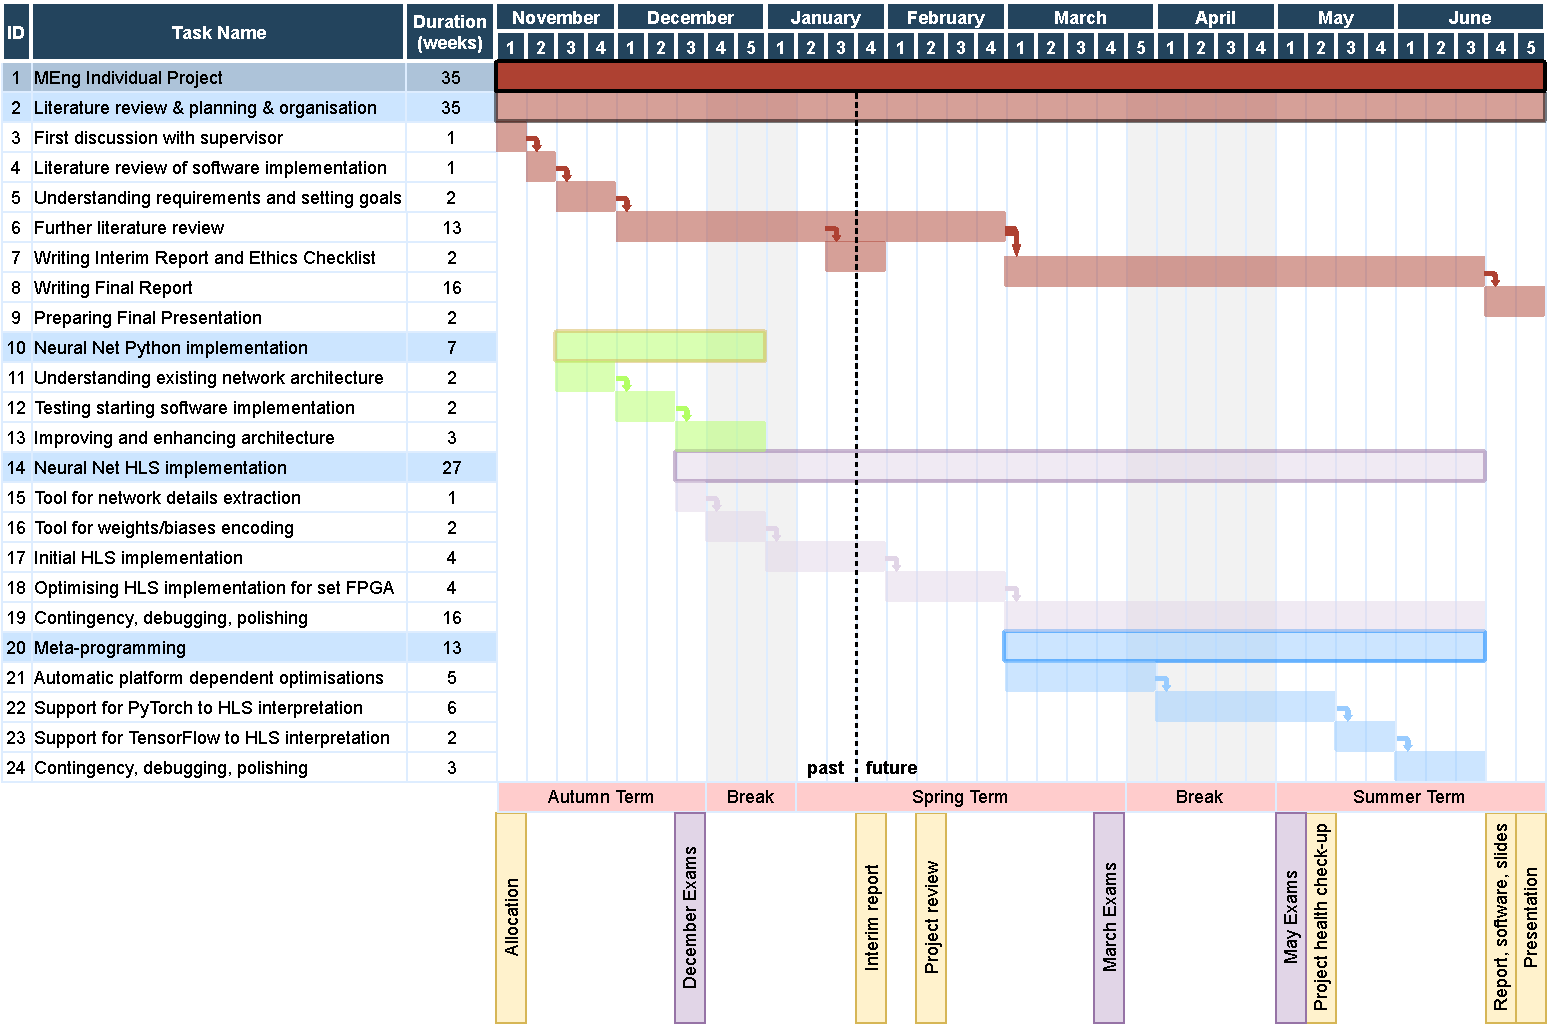
\includegraphics[trim={0cm 0cm 0cm 0cm}, width=1.2\textwidth, center]{project/gantt_chart.pdf}
  \caption{Project's Gantt chart representing initial plan of the work; past schedule has been updated to match ongoing progress accordingly}
  \label{fig:gantt-chart}
\end{figure}